\documentclass[11pt,]{article}
\usepackage{lmodern}
\usepackage{amssymb,amsmath}
\usepackage{ifxetex,ifluatex}
\usepackage{fixltx2e} % provides \textsubscript
\ifnum 0\ifxetex 1\fi\ifluatex 1\fi=0 % if pdftex
  \usepackage[T1]{fontenc}
  \usepackage[utf8]{inputenc}
\else % if luatex or xelatex
  \ifxetex
    \usepackage{mathspec}
  \else
    \usepackage{fontspec}
  \fi
  \defaultfontfeatures{Ligatures=TeX,Scale=MatchLowercase}
    \setmainfont[]{Georgia}
\fi
% use upquote if available, for straight quotes in verbatim environments
\IfFileExists{upquote.sty}{\usepackage{upquote}}{}
% use microtype if available
\IfFileExists{microtype.sty}{%
\usepackage{microtype}
\UseMicrotypeSet[protrusion]{basicmath} % disable protrusion for tt fonts
}{}
\usepackage[margin=0.5in]{geometry}
\usepackage{hyperref}
\hypersetup{unicode=true,
            pdfborder={0 0 0},
            breaklinks=true}
\urlstyle{same}  % don't use monospace font for urls
\usepackage{graphicx,grffile}
\makeatletter
\def\maxwidth{\ifdim\Gin@nat@width>\linewidth\linewidth\else\Gin@nat@width\fi}
\def\maxheight{\ifdim\Gin@nat@height>\textheight\textheight\else\Gin@nat@height\fi}
\makeatother
% Scale images if necessary, so that they will not overflow the page
% margins by default, and it is still possible to overwrite the defaults
% using explicit options in \includegraphics[width, height, ...]{}
\setkeys{Gin}{width=\maxwidth,height=\maxheight,keepaspectratio}
\IfFileExists{parskip.sty}{%
\usepackage{parskip}
}{% else
\setlength{\parindent}{0pt}
\setlength{\parskip}{6pt plus 2pt minus 1pt}
}
\setlength{\emergencystretch}{3em}  % prevent overfull lines
\providecommand{\tightlist}{%
  \setlength{\itemsep}{0pt}\setlength{\parskip}{0pt}}
\setcounter{secnumdepth}{0}
% Redefines (sub)paragraphs to behave more like sections
\ifx\paragraph\undefined\else
\let\oldparagraph\paragraph
\renewcommand{\paragraph}[1]{\oldparagraph{#1}\mbox{}}
\fi
\ifx\subparagraph\undefined\else
\let\oldsubparagraph\subparagraph
\renewcommand{\subparagraph}[1]{\oldsubparagraph{#1}\mbox{}}
\fi

%%% Use protect on footnotes to avoid problems with footnotes in titles
\let\rmarkdownfootnote\footnote%
\def\footnote{\protect\rmarkdownfootnote}

%%% Change title format to be more compact
\usepackage{titling}

% Create subtitle command for use in maketitle
\newcommand{\subtitle}[1]{
  \posttitle{
    \begin{center}\large#1\end{center}
    }
}

\setlength{\droptitle}{-2em}
  \title{}
  \pretitle{\vspace{\droptitle}}
  \posttitle{}
  \author{}
  \preauthor{}\postauthor{}
  \date{}
  \predate{}\postdate{}


\begin{document}

\hypertarget{itk-contributions}{%
\subsection{ITK contributions}\label{itk-contributions}}

\begin{itemize}
\item
  \textbf{Run-length matrices for texture analysis.} Texture analysis
  provides quantitative information describing properties in images
  (e.g., lung CT) such as coarseness and smoothness. Two common
  quantification schemes are based on co-occurence matrices and
  run-length matrices. Although the co-occurence measures are readily
  available in the Insight Toolkit, there were no such set of classes
  exists for run-length measures until our open-source implementation
  {[}1{]}. These classes have since been integrated into the toolkit.
\item
  \textbf{Class architecture for patch-based functionality.} In {[}2{]}
  and {[}3{]}, we introduced a complete framework for ITK classes based
  on patch-based algorithmic processing. This approach has demonstrated
  utility for processes such as denoising, joint label fusion, and
  super-resolution. This joint label fusion work (originally discussed
  in {[}4{]}) is the basis for our lung and lobe estimation framework
  {[}5{]}. Similarly, the denoising algorithm {[}6{]} features
  prominently in our preprocessing pipelines.
\end{itemize}

\hypertarget{antsrnet}{%
\subsubsection{ANTsRNet}\label{antsrnet}}

The recent interest in deep learning techniques and the associated
successes with respect to a variety of applications has motivated
adoption of such techniques within the medical imaging research
community. Basic image operations such as classification, object
identification, and segmentation (as well as more focused techniques)
has significant potential for facilitating basic medical research. In
light of these new developments, and in order to better meet the modern
needs of the community, we have modified this specific aim for ITK-Lung
to include the implementation and dissemination of open-source deep
learning architectures relevant to the use cases of our partner
investigators.

Towards this end, we have created \emph{ANTsRNet}--a collection of
well-known deep learning architectures ported to the R language.
ANTsRNet is built using the Keras neural network library (available
through R) and is highly integrated with the ANTsR package, the R
interface of the ANTs toolkit. Consistent with our other software
offerings, ongoing development is currently carried out on GitHub using
a well-commented coding style, thorough documentation, and
self-contained working examples.

It should be noted that various implementations of different deep
learning architectures exist and are largely available to the public.
However, we feel that this work fills an unmet need. Based on our own
search, many publicly available implementations, while functional, are
not developed with large-scale distribution and application as end
goals. There is little, if any, coding consistency between the various
implementations leading to non-standardized APIs and difficulties in
code navigation for debugging and/or didactic reasons. In addition, the
vast majority employ the Python language which is understandable given
its widespread usage by data scientists. However, this work makes these
powerful new developments available through a major platform heavily
used by statisticians and data scientists alike. In addition, the
R-based interface to the ANTs toolkit allows for preprocessing and data
augmentation strategies specific to medical imaging. As a result of
these current efforts, we were recently awarded a Titan XP GPU from the
NVIDIA corporation for facilitating ongoing development.

Although much work remains to be completed, we have made significant
progress. As noted below, several architectures have been implemented
for both 2-D and 3-D images spanning the broad application areas of
image classification, object detection, and image segmentation. It
should be noted that most reporting in the literature has dealt
exclusively with 2-D implementations. This is understandable due to
memory and computational speed constraints limiting practical 3-D
application on current hardware. However, given the importance that 3-D
data has for medical imaging and the rapid progress in hardware, we feel
it worth the investment in implementing corresponding 3-D architectures.
Each architecture is accompanied by one or more self-contained examples
for testing and illustrative purposes. In addtion, we have made novel
data augmentation strategies available to the user and illustrated them
with Keras-specific batch generators. These contributions are outlined
below.

\textbf{Image classification}

\begin{itemize}
\item
  \textbf{AlexNet.} Although convolutional neural networks (CNNs) have
  been around since the 1970s, it was the ImageNet competition of 2012
  and the superior results produced by the AlexNet architecture {[}7{]}
  that spurred its subsequent popularity such that CNNs are now the
  preferred approach to image-based neural networks. Although originally
  only 2-D, both 2-D and 3-D implementations have been implemented.
  Example test code employs the MNIST data set for classifying
  handwritten digits directly downloadable within R.
\item
  \textbf{Vgg16/Vgg19.} OxfordNet, or VGG, architectures {[}8{]} are
  much deeper than AlexNet and featured well in the 2014 ImageNet
  challenge. We implemented popular 16- and 19-layer versions for
  ANTsRNet. Given the simplicity and excellent performance, these form
  the classification component of such object detection architectures as
  the multibox Single-Shot Detection (SSD) network described below. Both
  2-D and 3-D versions have been implemented. Example test code employs
  the MNIST data set.
\item
  \textbf{GoogLeNet.} GoogLeNet, or Inception (version v3) {[}9{]}, is a
  22-layer network characterized by \emph{inception blocks} meant to
  reduce the number of parameters necessary to learn the targeted
  function. The architecture prevents a straightforward 3-D
  implementation so only a 2-D architecture is currently available.
  Example test code employs the MNIST data set.
\item
  \textbf{ResNet/ResNeXt.} The original ResNet architecture {[}10{]},
  along with a variant known as \emph{ResNeXt}{[}11{]}, is also included
  in ANTsRNet. ResNet, characterized by specialized blocks and skip
  connections, won the ImageNet challenge in 2015. Both 2-D and 3-D
  versions have been implemented. Example test code employs the MNIST
  data set.
\item
  \textbf{DenseNet.} The DenseNet architecture {[}12{]} is based on the
  observation that performance is typically enhanced with shorter
  connections between the layers and the input. This leads to an
  architecture in which every layer is connected to every other layer
  substantially reducing the number of parameters as well as other
  benefits. Both 2-D and 3-D versions have been implemented.
\end{itemize}

\textbf{Object detection}

\begin{itemize}
\tightlist
\item
  \textbf{SSD7/SSD300/SSD512.} A common preprocssing step in many
  medical imaging tsks is the localization of an object or region of
  interest. The Multibox Single-Shot Detection (SSD) algorithm is a
  well-known architecture with good performance {[}13{]}. We have
  implemented the original 2-D `300'- and `512'-style SSD networks in
  addition to their 3-D extensions. As these networks require
  significant training for determining optimal weighting, we also
  implemented a smaller architecture known as SSD7 which does not have
  such training data requirements. We also extended this architecture to
  3-D. A self-contained 2-D example of labeled faces demonstrates
  training and testing of the SSD7 architecture.
\end{itemize}

\textbf{Image segmentation}

\begin{itemize}
\tightlist
\item
  \textbf{U-Net/V-net.} Extending fully convolutional neural networks
  (fCNN) by including an upsampling decoding path with skip connections
  linking corresponding encoding/decoding layers, the authors of U-net
  {[}14{]} created a well-performing deep learning segmentation
  framework for 2-D images. This was later extended to 3-D with a custom
  Dice loss function in {[}15{]} denoted as V-net. Both 2-D and 3-D
  versions are implemented with a custom loss Dice function based on our
  work in the Insight Toolkit {[}16{]}. We have also created specialized
  decoding and encoding utilities for translating between ANTs images
  and data representations necessary for Keras operations. Examples
  include a left/right lung segmentation example which includes a
  demonstration of our unique template-based data augmentation strategy
  (see below).
\end{itemize}

\textbf{Template-based data augmentation}

In addition to these software contributions, a significant
methodological contribution we have made is the design of a
template-based data augmentation strategy. The need for large training
data sets is a well-known limitation associated with deep learning
algorithms. Whereas the architectures developed for such tasks as the
ImageNet competition have access to millions of annotated images, such
data access is not always is available and such is typically the case in
medical imaging. In order to achieve data set sizes necessary for
learning functional models, various data augmentation strategies have
been employed. These include application of intensity transformations,
such as brightening and enhanced contrast, and simple spatial
transformations, such as arbitrary rotations and translations. Regarding
the latter, such transformations are not ideal as they might not reflect
what is typically seen in medical images and might not sufficiently
sample the shape-space of the population currently being studied.

We currently use a template-based approach whereby image data sampled
from the population is used to construct a representative template that
is optimal in terms of both shape and intensity {[}17{]}. In addition to
the representative template, this template-building process yields the
transformations to/from each individual image to the template space.\\
This permits a propagation of the training data to the space of each
individual image. In the simplest case, the training data is used to
construct the template and then each individual training data is
propagated to the space of every other individual training data. In this
way, a training data set of size \(N\) can be expanded to a data set of
size \(N^2\) (cf Figure 1). A more complicated use case could build a
template from \(M\) data sets (where \(M > N\)). Transformations between
the training data and the template could then be used to propagate the
training data to the spaces of the individual members of the
template-generating data for an augmented data set size of
\(M \times N\).

\begin{figure}
\centering
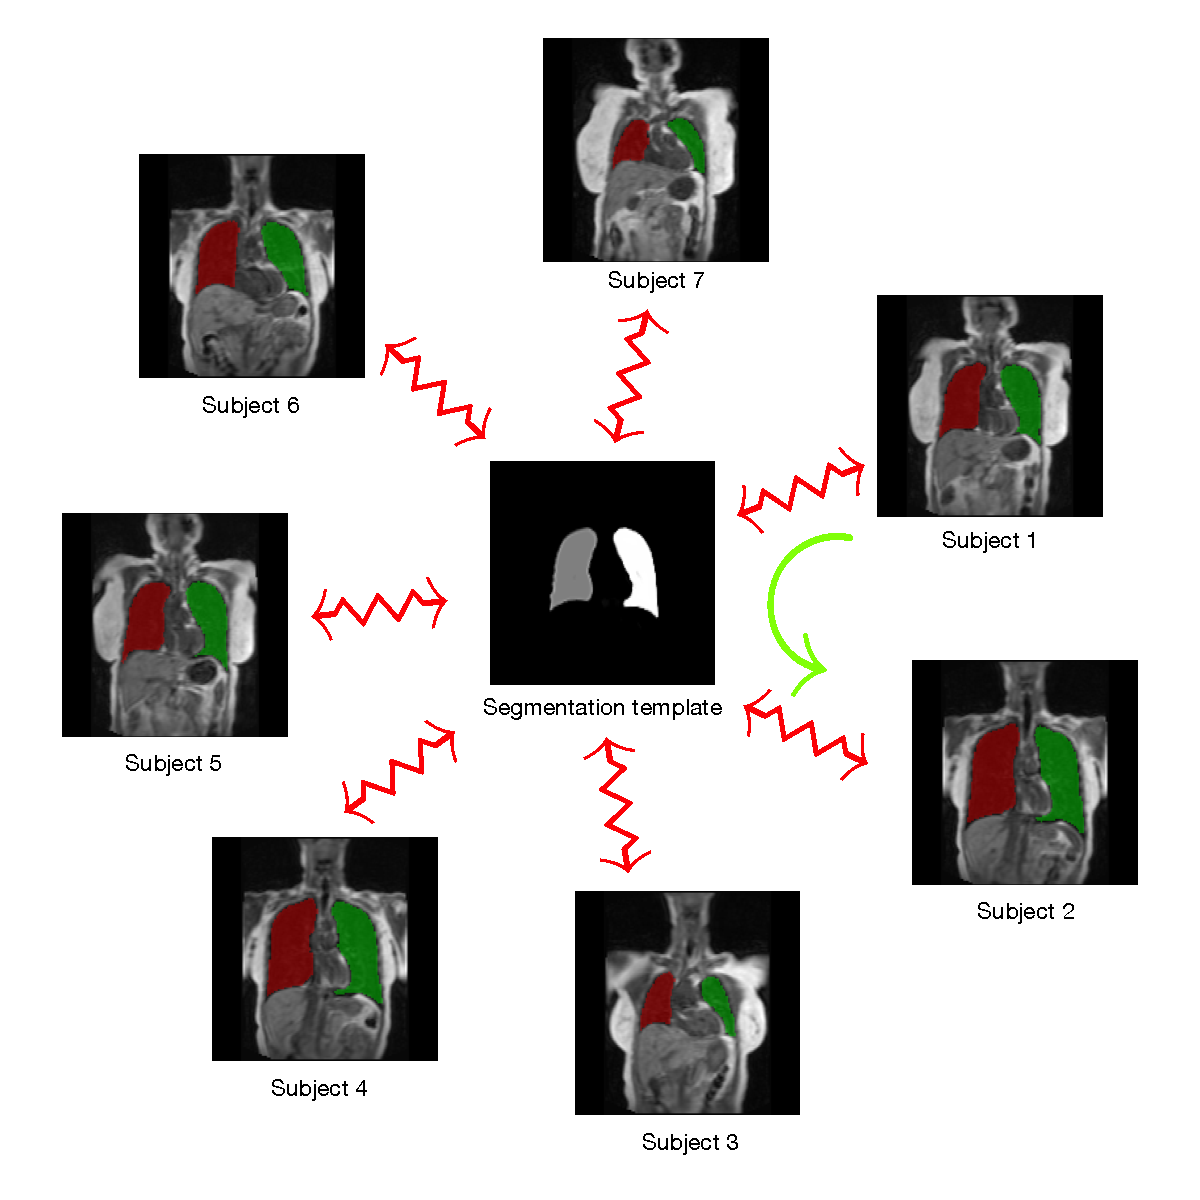
\includegraphics[width=\textwidth]{./Figures/DataAugmentation.pdf}
\caption{We introduce a novel data augmentation strategy for medical images using 
ANTs-based template construction.  Shown here is the 2-D U-net example where 
we create a template from the training data segmentation images where the 
foreground designates the left and right lungs.  This avoids the lack of 
internal correspondence while generating plausible global shape variations 
when mapping between individual training data.  We used 60+ images to 
create such a template permitting 60$^2$ = 3600 possible deformable shapes 
which can be further augmented by more conventional strategies (e.g., brightness
transformations, translations, etc.).}
\label{fig:augmentation}
\end{figure}

\newpage

\hypertarget{references}{%
\subsubsection*{References}\label{references}}
\addcontentsline{toc}{subsubsection}{References}

\hypertarget{refs}{}
\leavevmode\hypertarget{ref-tustison2008}{}%
1. Tustison, N. and Gee, J. ``\textbf{Run-Length Matrices for Texture
Analysis}'' \emph{Insight Journal} (2008):

\leavevmode\hypertarget{ref-tustison2017a}{}%
2. Tustison, N. and Manjon, J. ``\textbf{Two Luis Miguel Fans Walk into
a Bar in Nagoya ---\textgreater{} (Yada, Yada, Yada) ---\textgreater{}
an Itk-Implementation of a Popular Patch-Based Denoising Filter}''
\emph{Insight Journal} (2017):

\leavevmode\hypertarget{ref-tustison2017b}{}%
3. Tustison, N., Avants, B., Wang, H., Xie, L., Coupe, P., Yushkevich,
P., and Manjon, J. ``\textbf{A Patch-Based Framework for New Itk
Functionality: Joint Fusion, Denoising, and Non-Local
Super-Resolution}'' \emph{Insight Journal} (2017):

\leavevmode\hypertarget{ref-Wang:2013aa}{}%
4. Wang, H. and Yushkevich, P. A. ``\textbf{Multi-Atlas Segmentation
with Joint Label Fusion and Corrective Learning-an Open Source
Implementation}'' \emph{Front Neuroinform} 7, (2013): 27.
doi:\href{https://doi.org/10.3389/fninf.2013.00027}{10.3389/fninf.2013.00027}

\leavevmode\hypertarget{ref-Tustison:2016aa}{}%
5. Tustison, N. J., Qing, K., Wang, C., Altes, T. A., and Mugler, J. P.,
3rd. ``\textbf{Atlas-Based Estimation of Lung and Lobar Anatomy in
Proton Mri}'' \emph{Magn Reson Med} 76, no. 1 (2016): 315--20.
doi:\href{https://doi.org/10.1002/mrm.25824}{10.1002/mrm.25824}

\leavevmode\hypertarget{ref-Manjon:2010aa}{}%
6. Manjón, J. V., Coupé, P., Martí-Bonmatí, L., Collins, D. L., and
Robles, M. ``\textbf{Adaptive Non-Local Means Denoising of Mr Images
with Spatially Varying Noise Levels}'' \emph{J Magn Reson Imaging} 31,
no. 1 (2010): 192--203.
doi:\href{https://doi.org/10.1002/jmri.22003}{10.1002/jmri.22003}

\leavevmode\hypertarget{ref-Krizhevsky:2012}{}%
7. Krizhevsky, A., Sutskever, I., and Hinton, G. E. ``\textbf{ImageNet
Classification with Deep Convolutional Neural Networks}''
\emph{Proceedings of the 25th international conference on neural
information processing systems - volume 1} (2012): 1097--1105. Available
at \url{http://dl.acm.org/citation.cfm?id=2999134.2999257}

\leavevmode\hypertarget{ref-Simonyan:2014}{}%
8. Simonyan, K. and Zisserman, A. ``\textbf{Very Deep Convolutional
Networks for Large-Scale Image Recognition}'' \emph{CoRR} abs/1409.1556,
(2014): Available at \url{http://arxiv.org/abs/1409.1556}

\leavevmode\hypertarget{ref-Szegedy:2015}{}%
9. Szegedy, C., Vanhoucke, V., Ioffe, S., Shlens, J., and Wojna, Z.
``\textbf{Rethinking the Inception Architecture for Computer Vision}''
\emph{CoRR} abs/1512.00567, (2015): Available at
\url{http://arxiv.org/abs/1512.00567}

\leavevmode\hypertarget{ref-He:2015}{}%
10. He, K., Zhang, X., Ren, S., and Sun, J. ``\textbf{Deep Residual
Learning for Image Recognition}'' \emph{CoRR} abs/1512.03385, (2015):
Available at \url{http://arxiv.org/abs/1512.03385}

\leavevmode\hypertarget{ref-Xie:2016}{}%
11. Xie, S., Girshick, R. B., Dollár, P., Tu, Z., and He, K.
``\textbf{Aggregated Residual Transformations for Deep Neural
Networks}'' \emph{CoRR} abs/1611.05431, (2016): Available at
\url{http://arxiv.org/abs/1611.05431}

\leavevmode\hypertarget{ref-Huang:2016}{}%
12. Huang, G., Liu, Z., and Weinberger, K. Q. ``\textbf{Densely
Connected Convolutional Networks}'' \emph{CoRR} abs/1608.06993, (2016):
Available at \url{http://arxiv.org/abs/1608.06993}

\leavevmode\hypertarget{ref-Liu:2015}{}%
13. Liu, W., Anguelov, D., Erhan, D., Szegedy, C., Reed, S. E., Fu, C.,
and Berg, A. C. ``\textbf{SSD: Single Shot Multibox Detector}''
\emph{CoRR} abs/1512.02325, (2015): Available at
\url{http://arxiv.org/abs/1512.02325}

\leavevmode\hypertarget{ref-Ronneberger:2015}{}%
14. Ronneberger, O., Fischer, P., and Brox, T. ``\textbf{U-Net:
Convolutional Networks for Biomedical Image Segmentation}'' \emph{CoRR}
abs/1505.04597, (2015): Available at
\url{http://arxiv.org/abs/1505.04597}

\leavevmode\hypertarget{ref-Milletari:2016}{}%
15. Milletari, F., Navab, N., and Ahmadi, S. ``\textbf{V-Net: Fully
Convolutional Neural Networks for Volumetric Medical Image
Segmentation}'' \emph{CoRR} abs/1606.04797, (2016): Available at
\url{http://arxiv.org/abs/1606.04797}

\leavevmode\hypertarget{ref-tustison2009}{}%
16. Tustison, N. J. and Gee, J. C. ``\textbf{Introducing Dice, Jaccard,
and Other Label Overlap Measures to ITK}'' \emph{Insight Journal}
(2009):

\leavevmode\hypertarget{ref-Avants:2010aa}{}%
17. Avants, B. B., Yushkevich, P., Pluta, J., Minkoff, D., Korczykowski,
M., Detre, J., and Gee, J. C. ``\textbf{The Optimal Template Effect in
Hippocampus Studies of Diseased Populations}'' \emph{Neuroimage} 49, no.
3 (2010): 2457--66.
doi:\href{https://doi.org/10.1016/j.neuroimage.2009.09.062}{10.1016/j.neuroimage.2009.09.062}


\end{document}
